\subsection{All clips, one policy}
\label{sec:all}

We train one tracker and then one policy on all \tasksall{} tasks, with 8{,}192 training worlds. The credit rule now also spreads the worlds of each kind over the tasks.

\emph{The tracker.} After \fullTrackerSamples{} million samples the tracker succeeds from the clip start in \fullTrackerClip{} of episodes averaged over the tasks, and in \fullTrackerAway{} from displaced starts. It solves \fullTrackerSolved{} of the \tasksall{} tasks at 0.5 or better. The tasks it does not solve are mostly the tallest boxes and three clips whose climbs it never completes; a second stage of training on the partly solved tasks gained 0.01 per 25 million samples and was stopped.

\emph{The policy.} Fig.~\ref{fig:full} shows the policy trained with the credit rule and this tracker as its teacher. \fullSentence{}

\emph{Past the teacher.} Fig.~\ref{fig:fulltasks} shows where. \fullTasksSentence{} The rule's gate gives these tasks few reference worlds, because the teacher cannot show them; what solves them is the Boolean in goal worlds, on a policy that has learned to climb elsewhere. A tracker cannot do this: it has no goal to be rewarded for.

\begin{figure}[t]
\centering
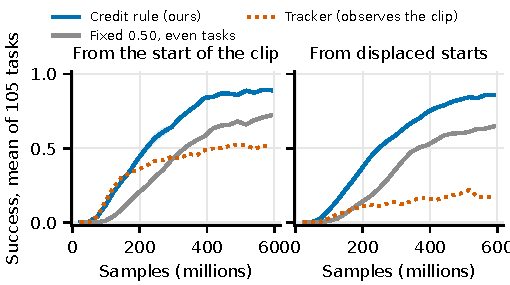
\includegraphics[width=\columnwidth]{figs/full_curves.pdf}
\caption{All \tasksall{} tasks, one policy. The policy does not observe a clip; the tracker that teaches it does. Credit rule: mean and range of \seedsAll{} seeds.}
\label{fig:full}
\end{figure}

\begin{figure*}[t]
\centering
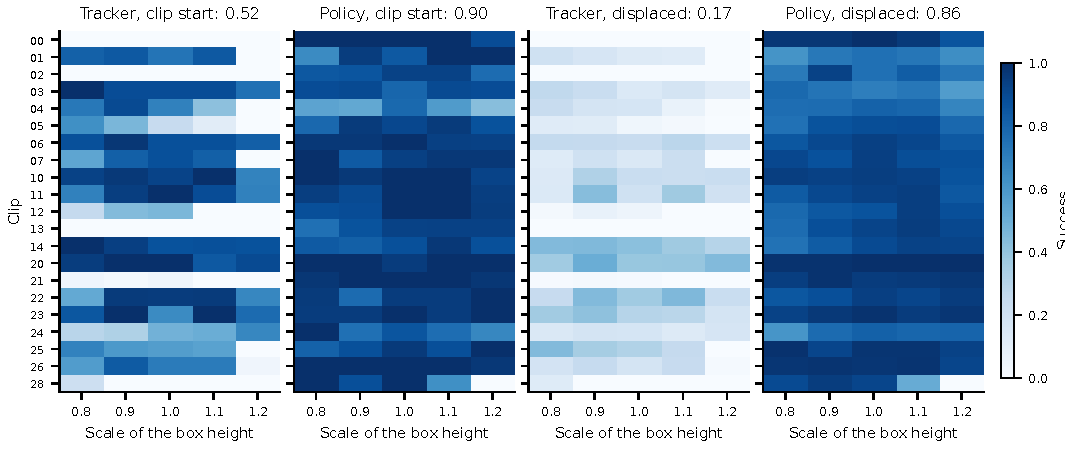
\includegraphics[width=\textwidth]{figs/full_tasks.pdf}
\caption{Success on every task at the end of training: a row per clip, a column per scale of the box height, and the mean over the tasks in each title. The policy is its first seed.}
\label{fig:fulltasks}
\end{figure*}

\subsection{Tasks that no world trained}

Does the policy climb boxes it never trained on? We repeat the run with tasks held out: no reference world and no goal world is ever placed on them, and the evaluation worlds still measure them (Table~\ref{tab:heldout}). \heldoutSentence{}

\begin{table}[t]
\centering
\caption{Tasks held out of training: no world of either kind is placed on them. Success averaged over the tasks.}
\label{tab:heldout}
\setlength{\tabcolsep}{4pt}
\begin{tabular}{@{}lccccc@{}}
\toprule
 & & \multicolumn{2}{c}{Tasks trained on} & \multicolumn{2}{c}{Tasks held out} \\
Held out of training & Tasks & clip & displaced & clip & displaced \\
\midrule
Two of five box heights & 42 & 0.87 & 0.80 & 0.90 & 0.81 \\
Five of 21 clips & 25 & 0.83 & 0.80 & 0.48 & 0.46 \\
\bottomrule
\end{tabular}

\end{table}

\subsection{Training time}

\timeSentence{}
